\section{Excercise 10}
Cho mạch sau. Tìm điện áp V. Bạn có thể làm điều này bằng mọi cách nhưng hãy nhớ
để giải thích nó một cách chi tiết. Sau đó mô phỏng mạch để kiểm tra kết quả.\\
\begin{figure}[!htbp]
    \centering
    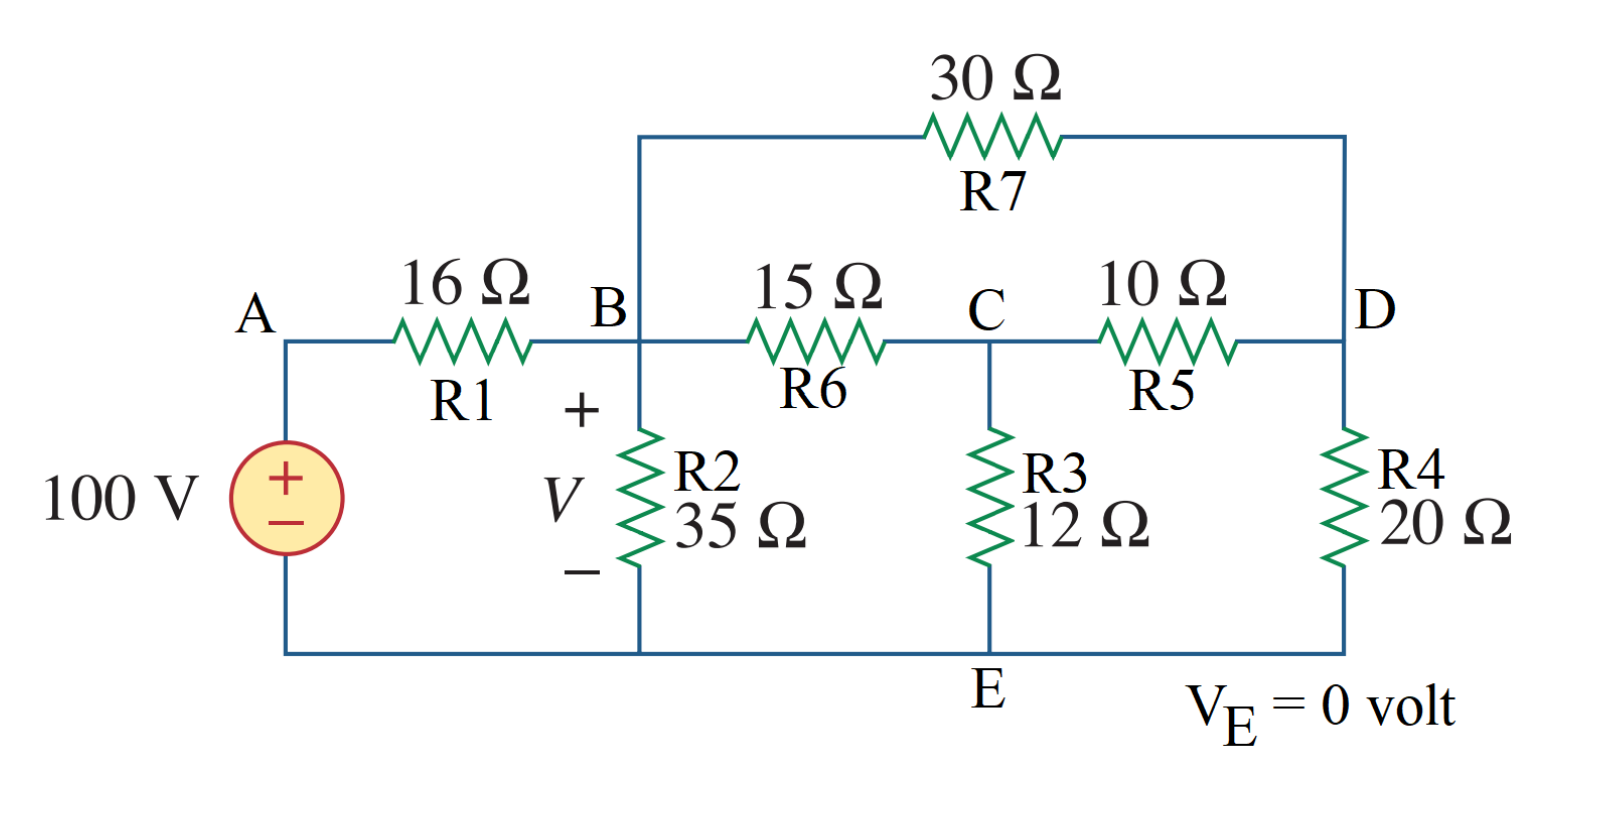
\includegraphics[width=0.7\textwidth]{graphics/ex10/f1.png}
    \caption{Tìm điện áp V}
\end{figure}
\textbf{Trả lời}\\
\begin{itemize}
    \item Biến đổi mạch về mạch đơn giản để tìm điện trở tương đương\\
    \begin{figure}[!htbp]
        \centering
        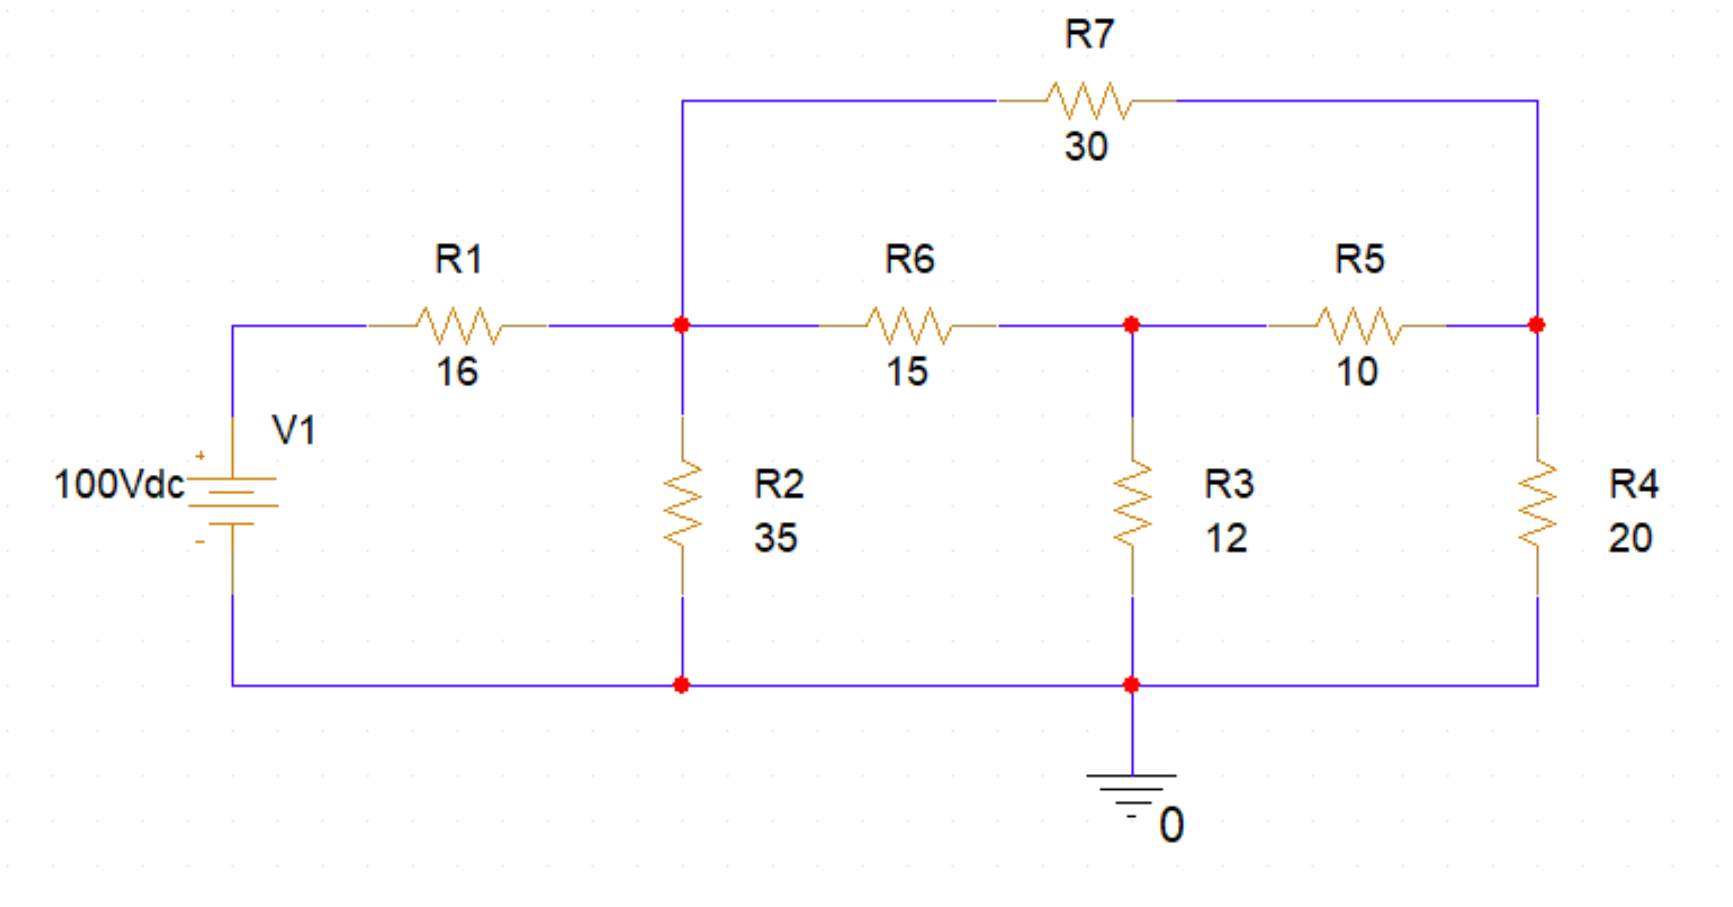
\includegraphics[width=0.7\textwidth]{graphics/ex10/f2.png}
        \caption{Mạch ban đầu}
        \end{figure}\\
        \begin{figure}[!htbp]
            \centering
            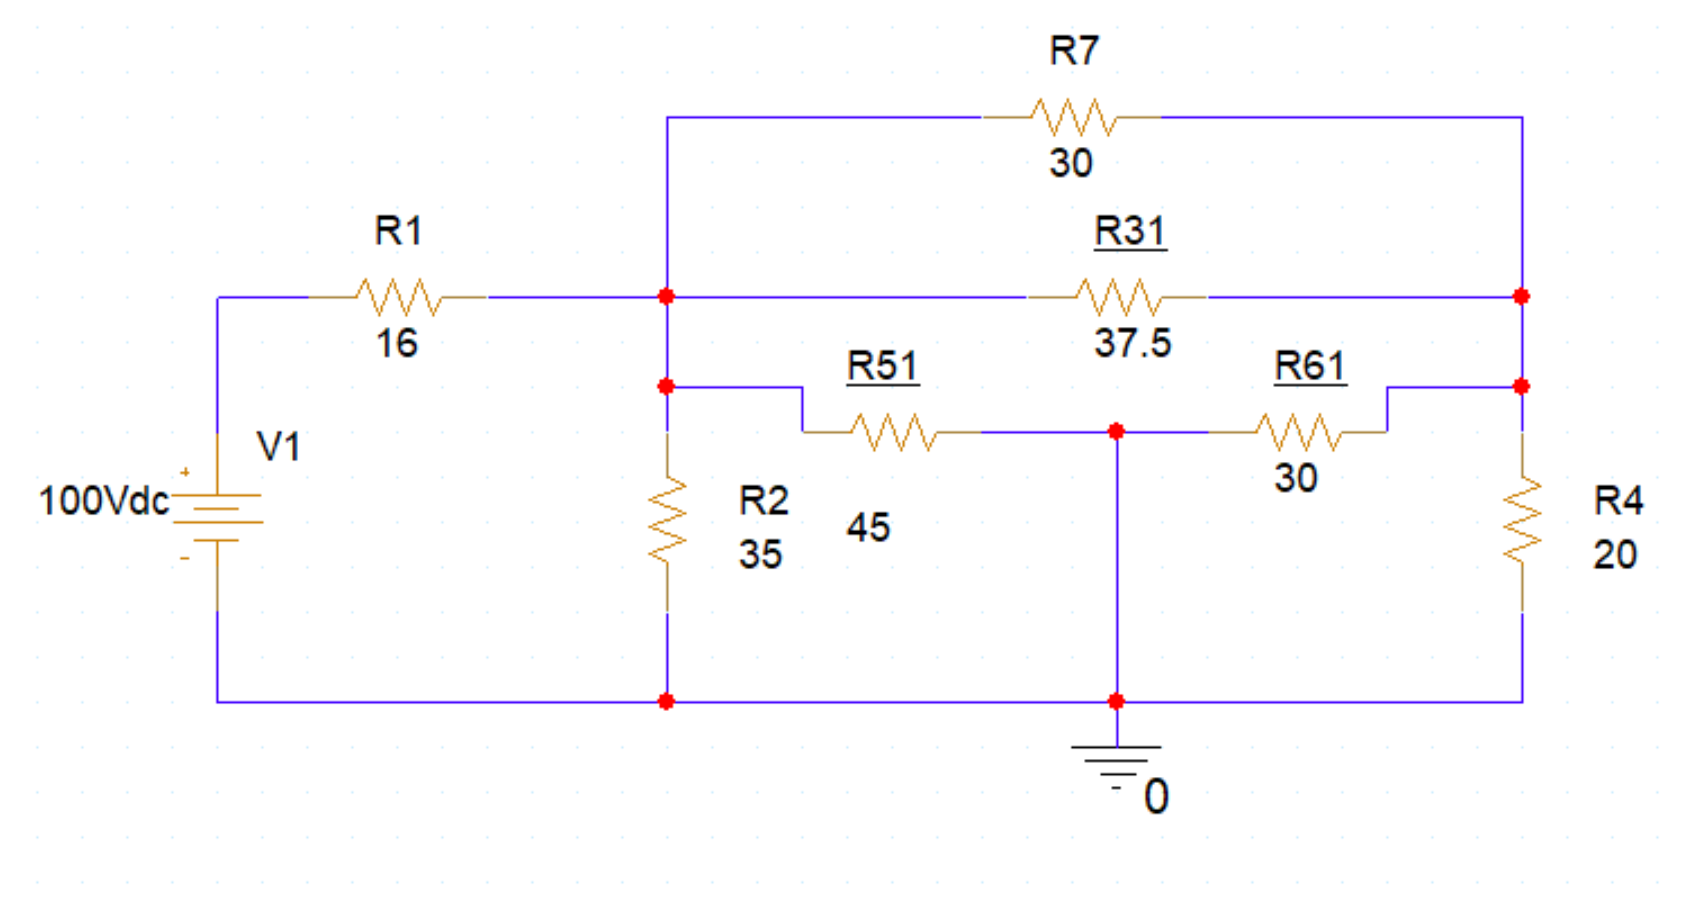
\includegraphics[width=0.7\textwidth]{graphics/ex10/f3.png}
            \caption{Dùng biến đổi wye-delta chuyển mạch wye \(R_3-R_5-R_6\) thành mạch delta \(R_{31}-R_{51}-R_{61}\)}
            \end{figure}\\
    Tính toán các giá trị:
    \begin{align*}
        R_{31} = \dfrac{R_3.R_5 + R_5.R_6 + R_6.R_3}{R_3} = 37,5 (\Omega).\\
        R_{51} = \dfrac{R_3.R_5 + R_5.R_6 + R_6.R_3}{R_5} = 45 (\Omega).\\
        R_{61} = \dfrac{R_3.R_5 + R_5.R_6 + R_6.R_3}{R_3} = 30 (\Omega).\\
    \end{align*}\\
    Tính toán các giá trị:
    \begin{align*}
        R_{31} // R_7 \rightarrow \dfrac{1}{R_{31\_7}} = \dfrac{1}{R_{31}} + \dfrac{1}{R_7} \rightarrow R_{31\_7} = 16,66667 (\Omega).\\
        R_{4} // R_{61} \rightarrow \dfrac{1}{R_{4\_61}} = \dfrac{1}{R_{61}} + \dfrac{1}{R_4} \rightarrow R_{4\_61} = 12 (\Omega).\\
    \end{align*}\\
    \begin{figure}[!htbp]
        \centering
        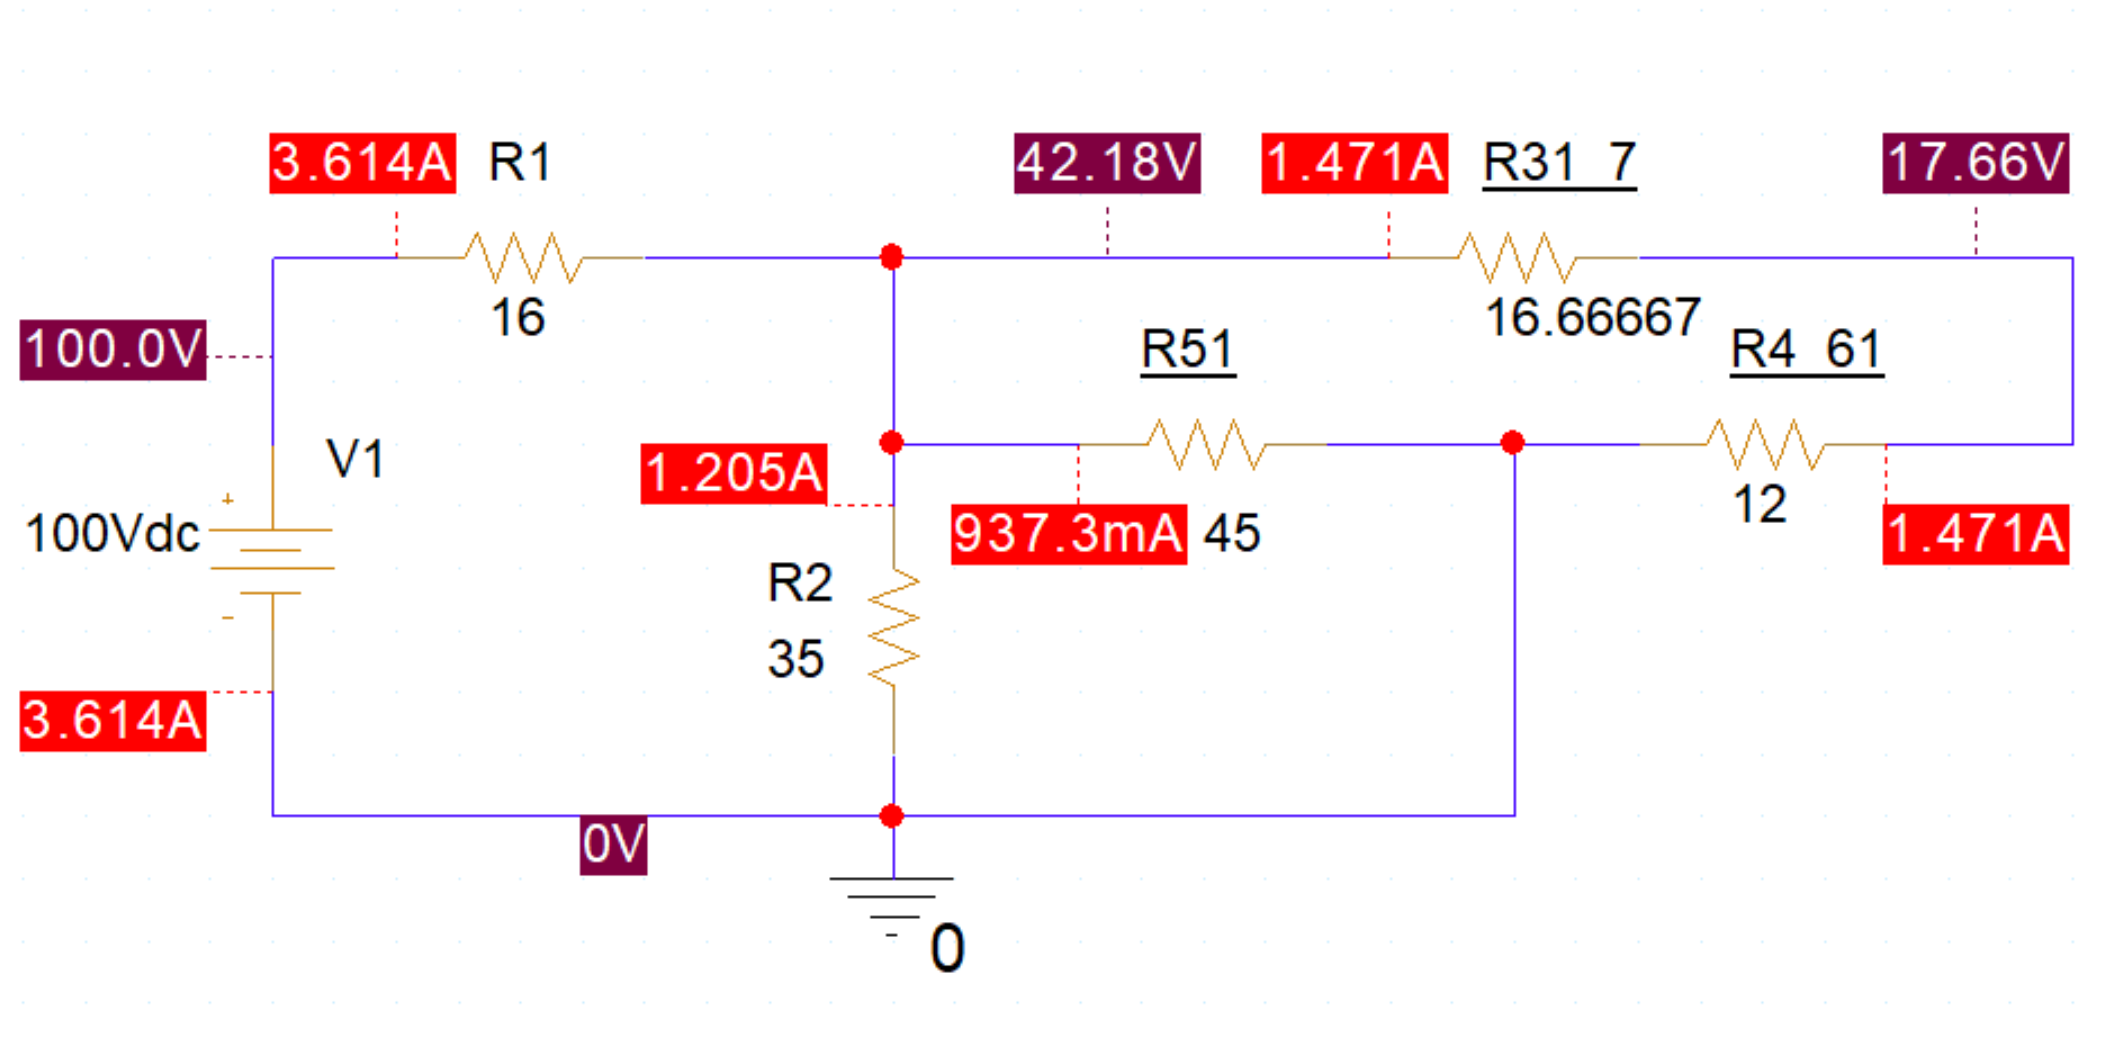
\includegraphics[width=0.7\textwidth]{graphics/ex10/f4.png}
        \caption{Biến đổi \(R_{61} // R_4\) thành \(R_{4\_61}\)}
        \end{figure}\\
        Tính toán các giá trị:\\
        \begin{align*}
            (R_{31\_7} nt R_{4\_61})//R_{51}//R_2 \rightarrow \dfrac{1}{R_n} = \dfrac{1}{R_{31\_7} + R_{4\_61}} + \dfrac{1}{R_{51}} + \dfrac{1}{R_2}
        \end{align*}
    \item 
\end{itemize}
